\documentclass[a4paper,14pt]{extreport}
  \usepackage[left=1.5cm,right=1.5cm,
      top=1.5cm,bottom=2cm,bindingoffset=0cm]{geometry}
  \usepackage{scrextend}
  \usepackage[T1,T2A]{fontenc}
  \usepackage[utf8]{inputenc}
  \usepackage[english,russian,ukrainian]{babel}
  \usepackage{tabularx}
  \linespread{1.5}
  \usepackage{amssymb}
  \usepackage{color}
  \usepackage{amsmath}
  \usepackage{mathrsfs}
  \usepackage{listings}
  \usepackage{graphicx}
  \graphicspath{ {./images/} }
  \usepackage{lipsum}
  \usepackage{xcolor}
  \usepackage{hyperref}
  \usepackage{tcolorbox}
  \usepackage{tikz}
  \usepackage[framemethod=TikZ]{mdframed}
  \usepackage{wrapfig,boxedminipage,lipsum}
  \mdfdefinestyle{MyFrame}{%
  linecolor=blue,outerlinewidth=2pt,roundcorner=20pt,innertopmargin=\baselineskip,innerbottommargin=\baselineskip,innerrightmargin=20pt,innerleftmargin=20pt,backgroundcolor=gray!50!white}
   \usepackage{csvsimple}
   \usepackage{supertabular}
  \usepackage{pdflscape}
  \usepackage{fancyvrb}
  %\usepackage{comment}
  \definecolor{ggreen}{rgb}{0.4,1,0}
  \definecolor{rred}{rgb}{1,0.1,0.1}
  \usepackage{array,tabularx}
  \usepackage{colortbl}

  \usepackage{varwidth}
  \tcbuselibrary{skins}
  \usepackage{fancybox}

  \definecolor{ggreen}{rgb}{0.4,1,0}
  \definecolor{rred}{rgb}{1,0.1,0.1}
  \definecolor{amber}{rgb}{1.0, 0.75, 0.0}
  \definecolor{babyblue}{rgb}{0.54, 0.81, 0.94}
  \definecolor{asparagus}{rgb}{0.53, 0.66, 0.42}
  \definecolor{chartreuse}{rgb}{0.5, 1.0, 0.0}
  \definecolor{darkorchid}{rgb}{0.6, 0.2, 0.8}
  \usepackage{fp}

  \usepackage{float}
  \usepackage{wrapfig}
  \usepackage{framed}
  %for nice Code{
  \lstdefinestyle{customc}{
    belowcaptionskip=1\baselineskip,
    breaklines=true,
    frame=L,
    xleftmargin=\parindent,
    language=C,
    showstringspaces=false,
    basicstyle=\small\ttfamily,
    keywordstyle=\bfseries\color{green!40!black},
    commentstyle=\itshape\color{purple!40!black},
    identifierstyle=\color{blue},
    stringstyle=\color{orange},
  }
  \lstset{escapechar=@,style=customc}
%}


\begin{document}

\newtcbox{\xmybox}[1][red]{on line, arc=7pt,colback=#1!10!white,colframe=#1!50!black, before upper={\rule[3pt] {0pt}{10pt}},boxrule=1pt,boxsep=0pt,left=6pt, right=6pt,top=2pt,bottom=2pt}


\pagecolor{white}
\begin{titlepage}
  \begin{center}
  \large
  Національний технічний університет України \\"Київський політехнічний інститут імені Ігоря Сікорського"


  Факультет Електроніки

  Кафедра мікроелектроніки
  \vfill

  \textsc{ЗВІТ}\\

  {\Large Про виконання прктичної №5\\
  з дисципліни: «Твердотільна електроніка-2»\\[1cm]

  }
  \bigskip
  \end{center}
  \vfill

  \newlength{\ML}
  \settowidth{\ML}{«\underline{\hspace{0.4cm}}» \underline{\hspace{2cm}}}
  \hfill
  \begin{minipage}{1\textwidth}
  Виконавець:\\
  Студент 3-го курсу \hspace{4cm} $\underset{\text{(підпис)}}{\underline{\hspace{0.2\textwidth}}}$  \hspace{1cm}А.\,С.~Мнацаканов\\
  \vspace{1cm}

  Перевірив: \hspace{6.1cm} $\underset{\text{(підпис)}}{\underline{\hspace{0.2\textwidth}}}$  \hspace{1cm}О.\,В.~Мачулянський\\

  \end{minipage}

  \vfill

  \begin{center}
  2021
  \end{center}
\end{titlepage}

%-------------------------------1
  \begin{center}
   \fbox{Характеристики та параметри логічних елементів. Основні логічні
    функції.}\\ \fbox{ Класифікація логічних ІМС}
  \end{center}
 
  Логічні елементи насамперед класифікують по тих логічним функцій. Логічні функції
  вивчаються в алгебрі логіки, илн булевої алгебри. вони представляють
  собою операції над логічними змінними, які позначимо А, В, С і т. д. В алгебрі логіки різні логічні вирази (висловлювання) можуть приймати тільки два значення: «істинно» чи «хибно». Для позначення істинності чи хибності висловлень використовують відповідно символи 1 чи 0. Кожна логічна змінна може приймати тільки одне значення: 1 або 0.\\

  Всі можливі логічні функції будь-якого числа логічних
  змінних можна утворити за допомогою трьох основних операцій: логічного заперечення (інверсії, операції НІ), логічного додавання (диз'юнкції, операції АБО) і логічного множення (кон'юнкції, операції І). Інверсія позначається знаком «-» над змінної, наприклад В = А. Логічна операція АБО для двох змінних А і В записується у вигляді С = А + В і визначається наступним чином: С = 1, якщо А == 1 або В = 1, або А = В =
  = 1. Логічна операція І для двох змінних А і В представляється як С = АВ, тобто С = 1 тільки в тому випадку, коли А = 1 і
  В = 1. Комбінація логічних операцій НІ і АБО призводить до більш складної функції АБО-НІ: С = А + В. У цьому випадку значення, що приймаються логічної змінної С, протилежні її значенням для операції АБО. Поєднання операцій НІ і І дає логічну функцію І-НІ: С = АВ.\\

  Логічні елементи, як правило, реалізують одну до з перерахованих вище функцій: НІ, І, АБО, І-НІ, АБО-НІ.
  Умовні графічні позначення ЛЕ, що виконують ці функції, представлені на рис. 1. Поєднуючи відповідним чином ці ЛЕ, можна отримати мікросхему, що виконує будь-яку більш складну логічну функцію. В принципі для цього досить використовувати тільки елементи І-НІ або АБО-НІ, тому вони набули найбільшого поширення в мікросхемах. Вище були наведені логічні функції двох змінних. Для їх виконання необхідні ЛЕ з двома входами (рис. 1, 6 - 9). При збільшенні числа логічних змінних відповідно зростає і число входів; їх може бути три, чотири і більше. Логічний елемент, що виконує
  операцію НІ (рис. 1, а), називається інвертором. Він має один вхід і один або кілька виходів. В останньому випадку для будь-якого з \ виходів виконується операція В, = - А (1 == 1,2, ..., \#).\\

  У більшості логічних елементів сучасних мікросхем логічні нулі (лог. 0) і одиниці (лог. 1) представляються двома істотно розрізняються значеннями напруги (потенціалу). Логічному нулю зазвичай відповідає напруга низького рівня(0, а логічній одиниці - напруга високого рівня 1).\\

  Логічні елементи по режиму роботи підрозділяють на
  статичні та динамічні. Статичні ЛЕ можуть працювати як в статичному, так і динамічному (імпульсному) режимах. Статичні елементи нанболее широко нспользуются в сучасних мікросхемах. Динамічні ЛЕ можуть працювати тільки в імпульсному режимі.\\

  Логічні елементи класифікують також типу використовуються в транзисторах. Найбільшого поширення отримали ЛЕ на біполярних і МДП-транзисторах. Крім того, інтенсивно розробляються ЛЕ на арсенід-галієвих МЕП і ГМЕП-транзисторах. Для кожного з перерахованих типів ЛЕ існує велика кількість їх схемотехнічних і конструктивно-технологічних різновидів. Наприклад, до біполярним ЛЕ відносяться елементи ТТЛ, емітерний-зв'язаної логіки (ЕСЛ), інтегральної инжекционной логіки (І * Л) і інші, розглянуті раніше.


  \begin{figure}[!h]
  \centering{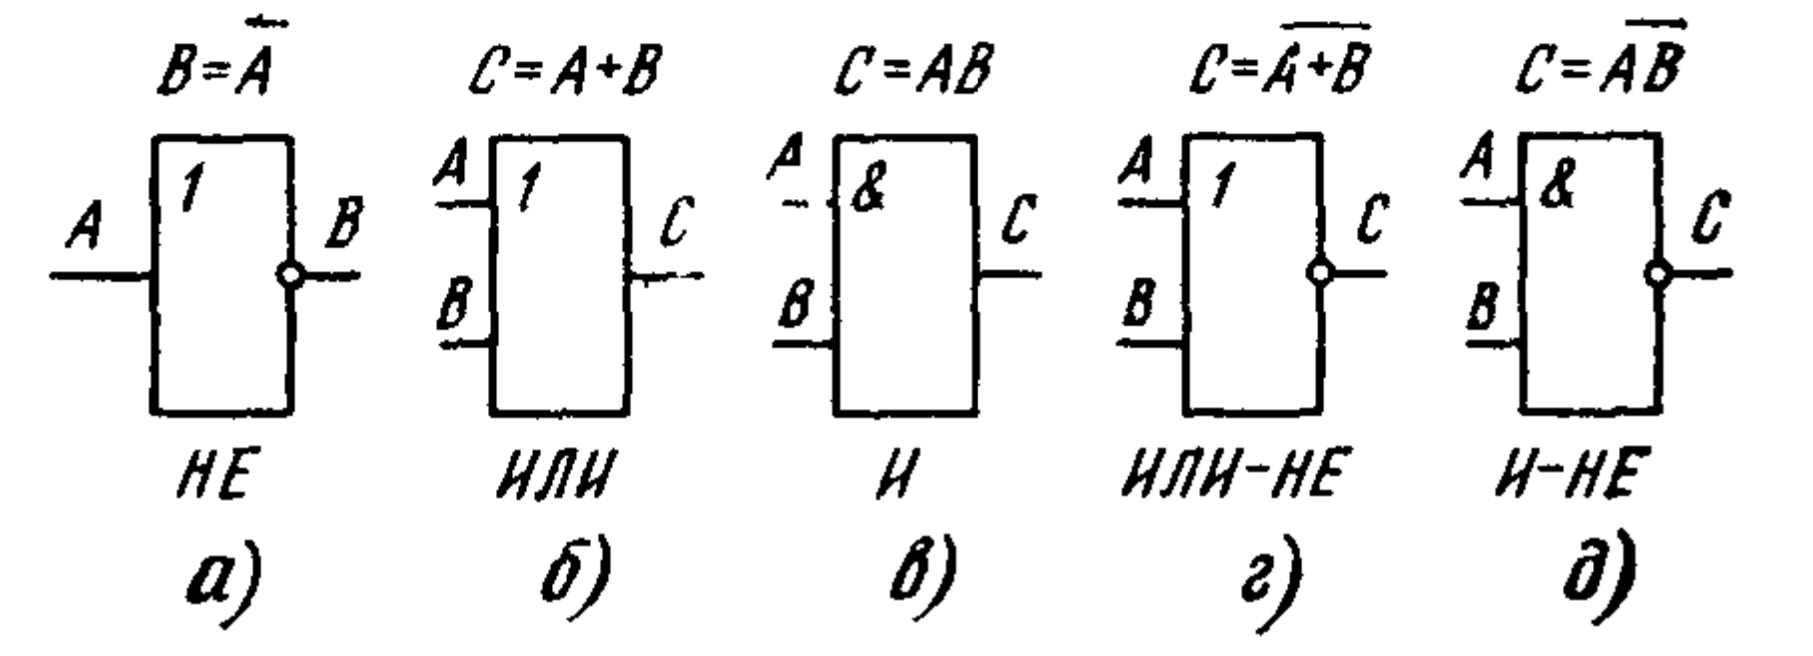
\includegraphics[width=0.8\textwidth]{1.png}}
  \end{figure}

  Основною статичною характеристикою ЛЕ є передаточна характеристика - залежність вихідної напруги  $U_{\text{вих}}$ від напруги на одному з входів при постійних напругах на інших входах, рівних $ U^0 $ або $ U^1 $
  і в залежності від типу ЛЕ. По виду передавальної характеристики розрізняють інвертують і неінвертуючий ЛЕ.На виході перших (НЕ, І-НЕ, АБО-НЕ
  ОІ та ін.) Отримують інверсні по отноше ІІ АОИ нию до вхідних логічні сигнали, на виходах друге (І, АБО та ін.)--- прямі.\\

  І В Передавальні характеристики инвертирующего і неинвертирующего ЛЕ представлені відповідно на рис. 2. Вони мають три чітко виражених ділянки. Ділянка 1 відповідає - станом $U_{\text{вих}}$ = $U_0$, ділянка 2 - станом - $U_{\text {вих}}$ = $U_1$. Крім того, є проміжна ділянка 3, на якій стан ЛЕ не визначений. У статичному режимі відповідні ділянки 3 значення напруг неприпустимі. Межі ділянок визначаються точками одиничного посилення, в яких виконується умова |
   $ dU_{\text{вих}}/dU_{\text{вх}}$ | = 1. Вхідні напруги, визна
  \begin{figure}[!h]
  \centering{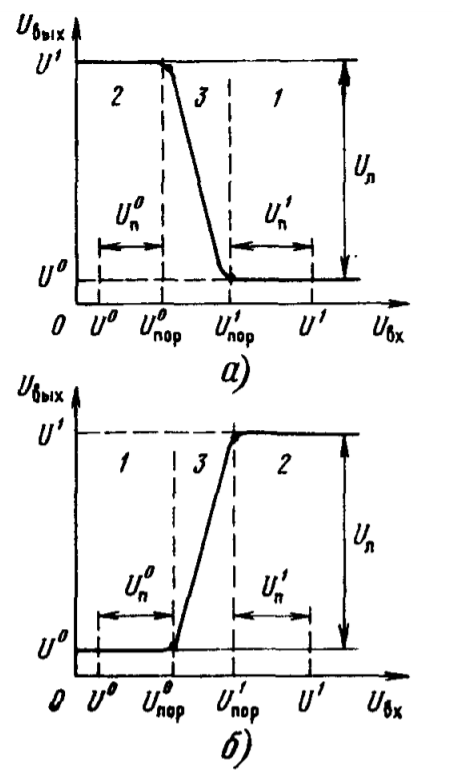
\includegraphics[width=0.4\textwidth]{2.png}}
  \end{figure}

  Складні логічні функції реалізуються за допомогою розгалужених ланцюгів, що складаються з ЛЕ. При цьому вихід одного ЛЕ з'єднують з
  входом іншого. Тому логічний сигнал $U^0$ або $U^1$ з виходу
  попереднього ЛЕ надходить на вхід наступного. Вхідні напруги $U^0$ або $U^1$, що задаються попередніми ЛЕ, показані на осях вхідних напруг на рис. 2.\\

  Крім логічних сигналів на входах можуть з'являтися напруги перешкоди, які або повищают, або знижують вхідна напруга. Якщо на вході діє напруга $U^0$, то небезпечні перешкоди, які мають позитивну полярність, так як вони підвищують вхідна напруга. При досить великій напрузі перешкоди робоча точка на передавальної характеристиці може зміститися в область
  перемикання 3 (див. рис. 2), що призведе до збою в роботі, т. е. помилковому зміни вихідних напруг в цифровому пристрої. При надходженні на вхід напруги І та напруги перешкоди отрицатель-
  ної полярності також можливо помилкове преключения. Максимально допустимі постійні напруги перешкоди позитивної полярності$U_{\text{п}}^0$ (при напрузі $U^0$ на вході) н негативної полярності (при напрузі$U^1$ на вході) визначають стійкість ЛЕ по
  відношенню до статичних (довготривалим) перешкод. Ці на напруги відзначені на рис. 2:

  $$U_{\text{п}}^0 = U_{\text{пор}}^0 - U_0$$

  $$U_{\text{п}}^1 = U^1 - U_{\text{пор}}^1$$

  Внутрішні перешкоди в цифровому пристрої возннкают прн пере-
  ключении ЛЕ, тому їх амплітуда пропорційна логічного перепаду Їх. Для оцінки завадостійкості ЛЕ крім напруг
  $U_{\text{п}}^0$ і $U_{\text{п}}^1$ використовують відносні величини

  $$k_{\text{п}}^0 = U_{\text{п}}^0/U_{\text{л}}$$
  $$k_{\text{п}}^1 = U_{\text{п}}^1/U_{\text{л}}$$
  звані коефіцієнтами завадостійкості. З рис. 2 від-
  але, що $k_{\text{п}}^0 + k_{\text{п}}^1$ <1, так як $U_{\text{п}}^0 + U_{\text{п}}^1$ < $k_{\text{п}}^0 + k_{\text{л}}$.\\

  Для підвищення завадостійкості необхідно збільшувати логічний перепад і зменшувати «ширину» області перемикання 3. \\

  Здатність навантаження п (коефіцієнт розгалуження на виході)
  характеризує максимальне число ЛЕ, аналогічних розглядається ті, які одночасно можна підключати до його виходу, чим
  вище здатність навантаження, тим менше число ЛЕ необхідно для
  побудови складної цифрової мікросхеми. Однак увелічеіне навантажувальної спроможності обмежена, оскільки з ростом числа навантажень погіршуються інші основні параметри ЛЕ, головним чином статична стійкість і швидкодія.
  Так, стійкість ЛЕ на біполярних транзнсторах зменшується з ростом числа навантажень, так як збільшуються вихідні струми в обох станах, а це призводить до зниження рівня напруги Е і підвищенню рівня напруги $U^1$. Середній час затримки сигналу зростає внаслідок збільшення ємності навантаження. З цієї причини до складу однієї серії мікросхем малої і середньої ступенів інтеграції і в цифрових пристроях БІС вводять ЛЕ з різною здатністю навантаження: п = 4 ... 25.\\

  Коефіцієнт об'єднання по входу т дорівнює числу входів ЛЕ.
  Зі збільшенням коефіцієнта т розширюються його логічні можливість ності за рахунок виконання функцій над ббльшім числом логічних змінних. При цьому для створення складного пристрою потрібно менше ЛЕ. Однак збільшення числа входів, як правило, погіршує інші основні параметри ЛЕ, перш за все швидкодію. для
  побудови більшості цифрових мікросхем досить мати елементи з числом входів m = 3 ... 4. Якщо потрібні схеми з підвищеним числом входів, то в серії мікросхем вводяться спеціальні ЛЕ расшірітелн числа входів.\\

  Температурні зміни електричних параметрів транзисторів, діодів і резисторів, використовуваних в ЛЕ, обумовлюють залежності них основних параметрів від температури. У зв'язкових з цим для
  мікросхем завжди задається діапазон робочих температур, в якому значення їх параметрів не виходять за певні межі.\\

  Важливу роль відіграють конструктивно-технологічні параметри
  і характеристики ЛЕ: площа, займана ЛЕ на кристалі (при заданому мінімальному топологічному розмірі), і кількість основних
  технологічних операцій, які використовуються при виготовленні мнкросхеми. Площа ЛЕ поряд з споживаної Мошность визначає максимально досяжну ступінь інтеграції, а кількість основних технологічних операцій - відсоток виходу придатних мікросхем і їх стонмость. Для зменшення площі ЛЕ прагнуть спростити їх ел-y схему, зменшити число використовуваних в ній транзисторів, діодів і резисторів. При проектуванні топології і структури ЛЕ для зниження його плошади зменшують число кишень, розміщуючи там,
  де це можливо, кілька транзисторів або резисторів в одній кишені. Використовують полікремнієві плівкові резистори, сформовані на поверхні кристала над транзисторами. Застосовуються поєднання областей транзисторів; в цьому випадку одна область кристал
  ла може використовуватися для декількох транзисторів, наприклад як база одного і колектор іншого біполярного транзистора.\\

  Для зіставлення ЛЕ різних типів при заданому рівні технологни, яке характеризується мінімальним топологічним розміром $\triangle$, використовують відносну площу, відображену числом квадратів зі стороною $\triangle$  (літографічних кваратів).
%-------------------------------2
  \begin{center}
    \fbox{Транзисторно-транзисторні ІМС.}
  \end{center}

  Відмітною ознакою елементів ТТЛ є многоеміттерного транзистор (див. 3.3), що входить у вхідному ланцюзі. Схема найпростішого елемента ТТЛ приведена на рис. 7.7. Вона містить вхідний двухеміттерний транзистор  
  $V T 1$ , в базовій ланцюга якого включений резистор $ R 1 $, і вихідний інвертор на транзисторі $ V T 2 $, в колекторної ланцюга якого включений резистор $ R $ . Многоеміттерного транзистор виконує логічну операцію І над вхідними логічними змінними $ A $ і $ B $, а на виході елемента реалізується функція І-НЕ:
  $ C = \overline{A B}. $ Найпростіші елементи ТТЛ використовують в Б І C.

  Розглянемо принцип дії ЛЕ в ст ати ч ес до м ре ж їм е, вважаючи, що він працює в складі ланцюжка послідовно з'єднаних однакових ЛЕ. Виділимо в цьому ланцюжку два сусідніх логічних елемента ЛЕ. і ЛЕ2 на рис. $ 7.8. $
    \begin{figure}[!h]
  \centering{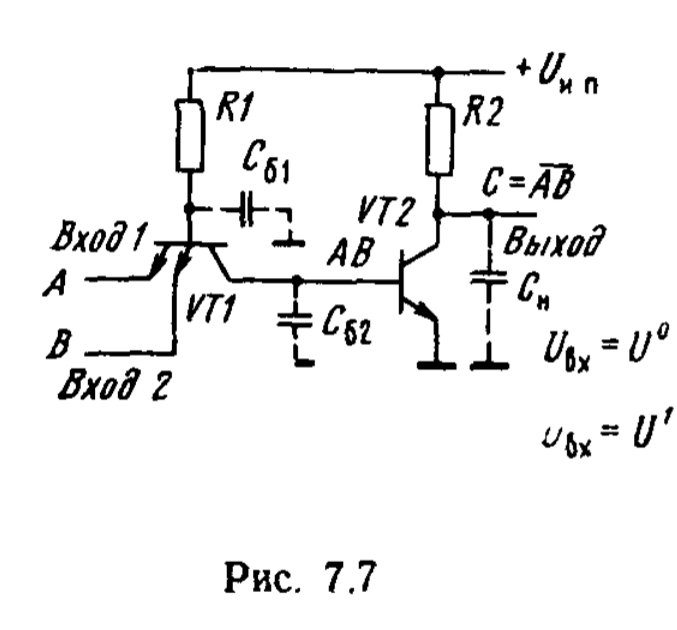
\includegraphics[width=0.6\textwidth]{3.png}}
  \end{figure}

  Нехай на перший вхід ЛЕ. подано напругу $ U^{0} $, а на другий напруга $ U^{1}. $ При цьому перший емітерний перехід зміщений в прямому напрямку, напруга на ньому позначимо $ U _{\text {БЕ1}}^{0}. $ Напруга на базі транзистора $ VT1 U _{\text {Б1}}^{0} =
   U _{\text {БЕ1}}^{0} + U^{0} $ ( близько $ 0,8 \text{~ B} $ при $ T=300 K)$.
     \begin{figure}[!h]
  \centering{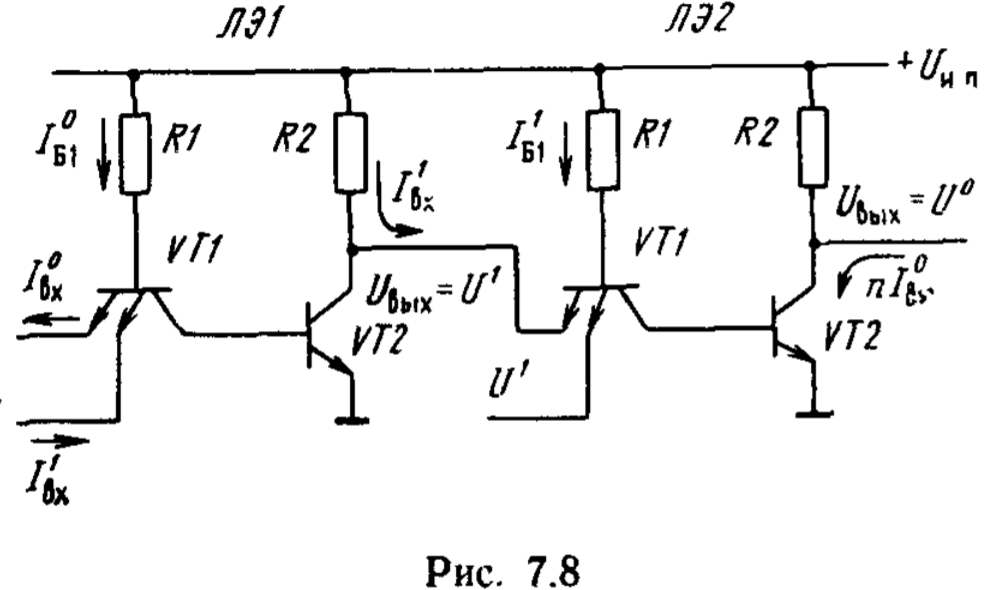
\includegraphics[width=0.6\textwidth]{4.png}}
  \end{figure}

  Цей струм випливає через перший вхід ЛЕ1. Другий емітерний перехід смещенв зворотному напрямку, тому через другий вхід втікає струм $ I _ {\text{sx}} ^ {1}. $ Цей струм також випливає через перший вхід. Тому струм першого входу $ I _ {\text{sx}} ^ {0} = I _ {\text{b} 1} ^ {0} + I _ {\text{sx}} ^ {1} $, а колекторний струм транзистора $ VT 1 $ (базовий струм транзистора $ VT 2) $ близький до нуля. Колекторний перехід транзистора $ VT 1 $ зміщений в прямому напрямку, а напруга між його колектором і першим емітером дорівнює напрузі насичення $ U _ {\text {Ке нас} 1 \text {для транзистора}} VT 1 $ при $ I _ {\text{ K}} \approx 0. $

  Напруга на базі транзистора $ VT 2 U _ {\text{b} \ni 2} ^ {0} = U ^ {0} + U _ {\text{K} \text {нас}} 1 $, що нижче його порогу відмикання $ U _ {\text {Бе пор2. }} $ Нагадаємо, що напруга $ U _ {\text {Бе пір на}} 2 \ldots 3 \varphi _ {\text{T}} $ нижче напруги база - емітер в режимі насичення [3]. Отже, транзистор $ V T 2 $ закритий і його колекторний струм близький до нуля. Через резистор $ R 2 $ в вихідний ланцюг ЛЕЕ 1 тече струм $ I _ {\text{Bx}} ^ {1} $, що є вхідним струмом для $ \underset {\Pi} {\Pi} \exists 2: I _ {\text{Bx}} ^ {1} = I _ {\text{b} 1} ^ {1} \beta_{l 1} $

  При малому струмі $ I_{\text{вх}}^{1} $ падіння напруги на резисторі 
  $ R 2 $ елемента ЛЕ1 невелика, тому напруга на виході ЛЕе відповідає напрузі високого рівня
  $$
  U ^ {1} = U_ {\text{ип}} -R_ {2} I _ {\text{sx}} ^ {1} = U _ {\text{H} \cdot \text{n}} - R_ { 2} I _ {\text{b}} ^ {1} \beta_ {I 1} \approx U _ {\text{u}. n}
  $$

  Одним із суттєвих недоліків найпростішого елемента ТТЛ (див. Рис. 7.7) є жорстке обмеження ємності навантаження: при великій $ C_ {\text {і}} $
   час наростання вихідної напруги визначається постійної часу $ R_ {2}
    C _ {\text {н }} $, з якої заряджається ця ємність. Для ЛЕ зі складним
     інвертором допустима значно велика ємність навантаження 
     $ \left (C _ {\text{n}} = 50 \ldots 150 \text{п} \Phi \right) $,
      оскільки вона заряджається великим емітерним струмом транзистора
       $ VT 4 $ , включається при виключенні транзистора $ \text{VT} 2 $.

  Споживана потужність для $ \pi \vartheta $ зі складним інвертором значно вище, ніж для простого, що обумовлено великою напругою джерела живлення. Крім того, складний інвертор споживає додаткову динамічну потужність при перемиканні: коли напруга на виході підвищується, транзистор $ V T 4 $ відкривається і його колекторний струм збільшує на цей час ток харчування. У ланцюзі харчування при перек.люченіі елемента зі стану $ U _ {\text {виx}} = U ^ {0} $ в стан $ U _ {\text {вих}} = U ^ {1} $ з'являється пік струму. Для його обмеження використовується резистор R4. Споживана потужність зростає при збільшенні робочої частоти перемикання.\\

  Логічний елемент зі складним інвертором в порівнянні з прос. Тейша займає значно більшу площу кристала. З цієї причини, а також внаслідок великої споживаної потужності його застосування обмежене цифровими мікросхемами малої і середньої ступенів інтеграції.

  Для підвищення швидкодії елементів ТТЛ в них використовують транзистори з діодом Шотки. Так, в схемі зі складним інвертором  всі транзистори, крім транзисторів VT4 і $ V T 5 $, що працюють в активному режимі, замінюють транзисторами з діодом Шотки. 
%-------------------------------3
  \begin{center}
  \fbox{Емітерно сполучена логіка; Інтегральна інжекційна логіка}
  \end{center}
  
  При $ U _ {\text{Bx}} = - U _ {\text{on}} $ обидва транзистора відкриті і працюють в активному режимі, їх еміттерние струми однакові і рівні $ 0,5 I _ {\ni}. $ Напруга на емітер $ U _ {\Theta} = - U _ {\text {оп}} - U _ {\text {Бе,}} ^ {\prime} $ де $ U _ {\text {Бе}} ^ {\prime} $ - пряма напруга на емітерний перехід, рівне $ 0,6. .0,7 \text{~ B} $ при $ T = 25 ^ {\circ} \text{C}. $ В активному режимі колекторний струм сушественно залежить від напруги $ U _ {\text {Бе:}} I _ {\text{K}} = \alpha I _ {\ni 0} \exp \left (U _ {\text {Бе}} / \varphi _ {\text {т}} \right). $ Відповідно до цієї формули зміна напруги $ U_ { \text {Бе}} $ на $ 2,3 \varphi _ {\text{r}} $ приводить до зміни струму на порядок. Якщо напруга на вході знизити на $ \delta U = 2,3 \varphi _ {\tau} $ (на 60 мВ при $ T = 25 {} ^ {\circ} \text{C} $) то колекторний струм вхідного транзистора стане значно менше струму опорного транзистора. При цьому напруга на виході 1 буBисогде випливає з $ \begin {array} {c} \text {ихід в навантаження при}  U _ {\text {ви х1}} \\\text {Колекторний}  \text {струм}  \text {опорного} \end {array} $ транзистора $ I _ {\text{K}} \approx \alpha I _ {\ni} \approx I _ {\ni.} $ Цей струм
  створює на резисторі $ R _ {\text{k}} $ падіння напруги, приблизно рівне $ R _ {\text{k}} I _ {\ni}. $ Тому напруга на другому виході відповідає напруга низького рівня $ U ^ {0} \approx - R_ {K} I _ {\ni} $









\end{document}
